
\documentclass[10pt]{article}
\usepackage{amsfonts,amsthm,amsmath,amssymb}
\usepackage{array}
\usepackage{epsfig}
\usepackage{fullpage}

%%% YOUR NAMES GO HERE %%%
\newcommand{\scribes}{Vahid Fazel-Rezai, Daniel Richman, Connor Sell}
%%% LECTURE NUMBER %%%
\newcommand{\lecnumber}{11}
%%% TITLE OF THE LECTURE %%%
\newcommand{\lectitle}{Semantically Secure Public-Key Encryption I
}
%%% DATE OF THE LECTURE %%%
\newcommand{\thedate}{Mar 9, 2016}

\begin{document}
%% Courtesy: Daniel Spielman, via Madhu Sudan --> Vinod Vaikuntanathan --> Aloni Cohen

%--------------
%% preamble.tex
%% this should be included with a command like
%% \input{preamble.tex}
%% \lecture{1}{September 4, 1996 }{Daniel A. Spielman}{name
%%  of poor scribe}


\hbadness=10000
\vbadness=10000

\newcommand{\handout}[6]{
   \renewcommand{\thepage}{#1 | Lec#6 | \arabic{page}}
   \noindent
   \begin{center}
   \framebox{
      \vbox{
    \hbox to 5.78in { {\bf #1}
     	 \hfill #2 }
       \vspace{4mm}
       \hbox to 5.78in { {\Large \hfill #5  \hfill} }
       \vspace{2mm}
       \hbox to 5.78in { {\it #3 \hfill #4} }
      }
   }
   \end{center}
   \vspace*{4mm}
}

\newcommand{\lecture}[4]{\handout{#1}{#2}{Lecturer:
#3}{Scribe: #4}{Lecture #1}}

\newtheorem{theorem}{Theorem}
\newtheorem{corollary}[theorem]{Corollary}
\newtheorem{lemma}[theorem]{Lemma}
\newtheorem{observation}[theorem]{Observation}
\newtheorem{proposition}[theorem]{Proposition}
\newtheorem{definition}[theorem]{Definition}
\newtheorem{claim}[theorem]{Claim}
\newtheorem{fact}[theorem]{Fact}
\newtheorem{assumption}[theorem]{Assumption}


%%%% GENERAL COMMANDS %%%%%%%%%%%%%%%%%%%%%%%%%%%%%%%%%


\newcommand{\dis}{\mathop{\mbox{\rm d}}\nolimits}
\newcommand{\per}{\mathop{\mbox{\rm per}}\nolimits}
\newcommand{\area}{\mathop{\mbox{\rm area}}\nolimits}
\newcommand{\cw}{\mathop{\rm cw}\nolimits}
\newcommand{\ccw}{\mathop{\rm ccw}\nolimits}
\newcommand{\DIST}{\mathop{\mbox{\rm DIST}}\nolimits}
\newcommand{\OP}{\mathop{\mbox{\it OP}}\nolimits}
\newcommand{\OPprime}{\mathop{\mbox{\it OP}^{\,\prime}}\nolimits}
\newcommand{\ihat}{\hat{\imath}}
\newcommand{\jhat}{\hat{\jmath}}
\newcommand{\abs}[1]{\mathify{\left| #1 \right|}}


%%%%% PROOF ENVIRONMENTS %%%%%%%%%%%%%%%%%%%%%%%%%%%%%%%%%%%%%%%%%%%%%%%%%%%%%%%%%%%%

\newenvironment{proof-sketch}{\noindent{\bf Sketch of Proof}\hspace*{1em}}{\qed\bigskip}
\newenvironment{proof-idea}{\noindent{\bf Proof Idea}\hspace*{1em}}{\qed\bigskip}
\newenvironment{proof-of-lemma}[1]{\noindent{\bf Proof of Lemma #1}\hspace*{1em}}{\qed\bigskip}
\newenvironment{proof-attempt}{\noindent{\bf Proof Attempt}\hspace*{1em}}{\qed\bigskip}
\newenvironment{proofof}[1]{\noindent{\bf Proof}
of #1:\hspace*{1em}}{\qed\bigskip}
\newenvironment{remark}{\noindent{\bf Remark}\hspace*{1em}}{\bigskip}

% \makeatletter
% \@addtoreset{figure}{section}
% \@addtoreset{table}{section}
% \@addtoreset{equation}{section}
% \makeatother

\newcommand{\FOR}{{\bf for}}
\newcommand{\TO}{{\bf to}}
\newcommand{\DO}{{\bf do}}
\newcommand{\WHILE}{{\bf while}}
\newcommand{\AND}{{\bf and}}
\newcommand{\IF}{{\bf if}}
\newcommand{\THEN}{{\bf then}}
\newcommand{\ELSE}{{\bf else}}

% \renewcommand{\thefigure}{\thesection.\arabic{figure}}
% \renewcommand{\thetable}{\thesection.\arabic{table}}
% \renewcommand{\theequation}{\thesection.\arabic{equation}}

\makeatletter
\def\fnum@figure{{\bf Figure \thefigure}}
\def\fnum@table{{\bf Table \thetable}}
\long\def\@mycaption#1[#2]#3{\addcontentsline{\csname
  ext@#1\endcsname}{#1}{\protect\numberline{\csname
  the#1\endcsname}{\ignorespaces #2}}\par
  \begingroup
    \@parboxrestore
    \small
    \@makecaption{\csname fnum@#1\endcsname}{\ignorespaces #3}\par
  \endgroup}
\def\mycaption{\refstepcounter\@captype \@dblarg{\@mycaption\@captype}}
\makeatother


\newcommand{\figcaption}[1]{\mycaption[]{#1}}
\newcommand{\tabcaption}[1]{\mycaption[]{#1}}
\newcommand{\head}[1]{\chapter[Lecture \##1]{}}
\newcommand{\mathify}[1]{\ifmmode{#1}\else\mbox{$#1$}\fi}
%\renewcommand{\Pr}[1]{\mathify{\mbox{Pr}\left[#1\right]}}
%\newcommand{\Exp}[1]{\mathify{\mbox{Exp}\left[#1\right]}}
\newcommand{\bigO}O
\newcommand{\set}[1]{\mathify{\left\{ #1 \right\}}}
\def\half{\frac{1}{2}}


% Command that ignores input.
\newcommand{\remove}[1]{}
\newcommand{\ignore}[1]{}
\newenvironment{ignoreme}{\ignore{}{}}

%%%%%%%%%%%%%% LATTICES %%%%%%%%%%%%%%%%%%%%%%%%%%%%%%%%%%%%%%%%%%%%%%%%%%%%%%%%%


\def\hh{\sigma^{\text{\rm\tiny top}}}
\def\ph{\sigma^{\text{\rm\tiny bot}}}
\def\hM{M^{\text{\rm\tiny top}}}
\def\pM{M^{\text{\rm\tiny bot}}}
\def\lsb{\mathsf{lsb}}

\newcommand{\gapSVP}{\mathsf{gapSVP}}
\newcommand{\SIVP}{\mathsf{SIVP}}

\def\dlwe{\mathsf{DLWE}}


\def\Zp{\Z_p}
\newcommand{\ip}[1]{\langle #1 \rangle}
\def\Psibar{\overline{\Psi}}

%Security Parameter
\newcommand{\secparam}{\kappa}
\newcommand{\secp}{\secparam}

\newcommand{\svp}{\mathsf{SVP}}

% Vectors, Matrices and such

\def\veca{\vc{a}}
\def\vecb{\vc{b}}
\def\vecc{\vc{c}}
\def\vecd{\vc{d}}
\def\vece{\vc{e}}
\def\vecm{\vc{m}}
\def\vecs{\vc{s}}
\def\vect{\vc{t}}
\def\vecv{\vc{v}}
\def\vecx{\vc{x}}
\def\vecy{\vc{y}}

\def\Z{\mathbb{Z}}
\def\R{\mathbb{R}}
\def\Q{\mathbb{Q}}

% Changing QED symbol in claim proofs
\newenvironment{claimproof}{\begin{proof}
\renewcommand{\qedsymbol}{{$\blacksquare$}}
}{\end{proof}}

% Calligraphic and blackboard type letters.

\def\cA{{\cal A}}
\def\cB{{\cal B}}
\def\cC{{\cal C}}
\def\cD{{\cal D}}
\def\cE{{\cal E}}
\def\cF{{\cal F}}
\def\cG{{\cal G}}
\def\cH{{\cal H}}
\def\cI{{\cal I}}
\def\cJ{{\cal J}}
\def\cK{{\cal K}}
\def\cL{{\cal L}}
\def\cM{{\cal M}}
\def\cN{{\cal N}}
\def\cO{{\cal O}}
\def\cP{{\cal P}}
\def\cQ{{\cal Q}}
\def\cR{{\cal R}}
\def\cS{{\cal S}}
\def\cT{{\cal T}}
\def\cU{{\cal U}}
\def\cV{{\cal V}}
\def\cW{{\cal W}}
\def\cX{{\cal X}}
\def\cY{{\cal Y}}
\def\cZ{{\cal Z}}
%%%%%%%%%%%%%%%%%
\def\bbC{{\mathbb C}}
\def\bbE{{\mathbb E}}
\def\bbF{{\mathbb F}}
\def\bbG{{\mathbb G}}
\def\bbM{{\mathbb M}}
\def\bbN{{\mathbb N}}
\def\bbQ{{\mathbb Q}}
\def\bbR{{\mathbb R}}
\def\bbV{{\mathbb V}}
\def\bbZ{{\mathbb Z}}

\def\Zq{\bbZ_q}

%%%%%%%%%%%%%%%%%


% Rounding commands

\newcommand{\ceil}[1]{\left\lceil #1 \right\rceil}
\newcommand{\floor}[1]{\left\lfloor #1 \right\rfloor}
\newcommand{\round}[1]{\left\lfloor #1 \right\rceil}


% Other short-hands

\def\binset{\{0,1\}}
\def\pmset{\{\pm 1\}}
\def\ind{\mathbbm{1}}
%\def\ind{\mathbf{1}}

\newcommand{\norm}[1]{\left\| {#1} \right\|}
\newcommand{\norminf}[1]{\left\| {#1} \right\|_{\infty}}


% Assignments
\def\getsr{\stackrel{\scriptscriptstyle{\$}}{\gets}}
\def\getsd{{:=}}
%\def\bydef{\stackrel{.}{=}}
\def\bydef{\triangleq}
\def\getsf{{\gets}}



% Asymptotics

\def\poly{{\rm poly}}
\def\polylog{{\rm polylog}}
\def\polyloglog{{\rm polyloglog}}
\def\negl{{\rm negl}}
\newcommand{\ppt}{\mbox{{\sc ppt}}}
\def\Otilde{\widetilde{O}}

% Indistinguishability
\newcommand{\cind}{{\ \stackrel{c}{\approx}\ }}
\newcommand{\sind}{{\ \stackrel{s}{\approx}\ }}

% Complexity classes

\def\NP{\mathbf{NP}}
\def\Ppoly{{\mathbf{P}/\poly}}


% Cryptographic assumptions

\newcommand{\ddh}{\mathrm{DDH}}
\newcommand{\cdh}{\mathrm{CDH}}
\newcommand{\dlin}{\text{\rm $d$LIN}}
\newcommand{\lin}{\text{\rm Lin}}
\newcommand{\sxdh}{\mathrm{SXDH}}
\newcommand{\rsa}{\mathrm{RSA}}
\newcommand{\sis}{\mathrm{SIS}}
\newcommand{\isis}{\mathrm{ISIS}}
\newcommand{\lwe}{\mathsf{LWE}}
\newcommand{\qr}{\mathrm{QR}}


% Types of attacks

\newcommand{\adv}{\mathrm{Adv}}
\newcommand{\dst}{\mathrm{Dist}}
\newcommand{\leak}{\mathrm{Leak}}
\newcommand{\forge}{\mathrm{Forge}}
\newcommand{\col}{\mathrm{Col}}
\newcommand{\invt}{\mathrm{Inv}}
\newcommand{\cpa}{\text{\rm CPA}}
\newcommand{\kdm}{\mathrm{KDM}}
\newcommand{\kdi}{\mathrm{KDM}^{(1)}}
\newcommand{\kdmn}{\mathrm{KDM}^{(\usr)}}
\newcommand{\ibe}{\mathrm{IBE}}
\newcommand{\good}{\mathrm{GOOD}}
\newcommand{\legal}{\mathrm{L}}


% Quadratic residuosity related

\newcommand{\qrs}{\mathbb{QR}}
\newcommand{\js}{\mathbb{J}}


% Linear algebra

\newcommand{\mx}[1]{\mathbf{{#1}}}
\newcommand{\vc}[1]{\mathbf{{#1}}}
\newcommand{\gvc}[1]{\bm{{#1}}}
%\newcommand{\vc}[1]{\gvc{{#1}}}

\newcommand{\rk}{\text{\rm Rk}}
\newcommand{\spn}{\text{\rm Span}}

% Probability

\newcommand{\Ex}{\mathop{\bbE}}
\newcommand{\cov}{\mathop{\text{\rm Cov}}}

%\newcommand{\sd}{\mathop{\text{\tt dist}}}
\newcommand{\sd}{\mathop{\Delta}}


% Entropy

\newcommand{\mH}{\mathbf{H_{\infty}}}
\newcommand{\avgmH}{\mathbf{\widetilde{H}_{\infty}}}


% Cryptographic elements

\newcommand{\pk}{{pk}}
\newcommand{\evk}{{evk}}
\newcommand{\pp}{{pp}}
\newcommand{\sk}{{sk}}
\newcommand{\vk}{{vk}}
\newcommand{\td}{{td}}

\newcommand{\msk}{{msk}}
\newcommand{\id}{{id}}

\newcommand{\crs}{\text{\sf crs}}

\newcommand{\params}{{params}}
\newcommand{\state}{{setupstate}}

\newcommand{\query}{{query}}
\newcommand{\qstate}{{qstate}}
\newcommand{\resp}{{resp}}


% Algorithms


\newcommand{\keygen}{\mathsf{Keygen}}
\newcommand{\gen}{\mathsf{Gen}}
\newcommand{\eval}{\mathsf{Eval}}
\newcommand{\setup}{\mathsf{Setup}}
\newcommand{\extract}{\mathsf{Extract}}
\newcommand{\enc}{\mathsf{Enc}}
\newcommand{\dec}{\mathsf{Dec}}

\newcommand{\symname}{\mathsf{SYM}}
\newcommand{\symkeygen}{\mathsf{SYM.Keygen}}
\newcommand{\symgen}{\symkeygen}
\newcommand{\symenc}{\mathsf{SYM.Enc}}
\newcommand{\symdec}{\mathsf{SYM.Dec}}


\newcommand{\shname}{\mathsf{SH}}
\newcommand{\shkeygen}{\mathsf{SH.Keygen}}
\newcommand{\shgen}{\shkeygen}
\newcommand{\shenc}{\mathsf{SH.Enc}}
\newcommand{\shdec}{\mathsf{SH.Dec}}
\newcommand{\sheval}{\mathsf{SH.Eval}}

\newcommand{\hename}{\mathsf{HE}}
\newcommand{\hekeygen}{\mathsf{HE.Keygen}}
\newcommand{\hegen}{\hekeygen}
\newcommand{\heenc}{\mathsf{HE.Enc}}
\newcommand{\hedec}{\mathsf{HE.Dec}}
\newcommand{\heeval}{\mathsf{HE.Eval}}


\newcommand{\fhname}{\mathsf{FH}}
\newcommand{\fhkeygen}{\mathsf{FH.Keygen}}
\newcommand{\fhenc}{\mathsf{FH.Enc}}
\newcommand{\fhdec}{\mathsf{FH.Dec}}
\newcommand{\fheval}{\mathsf{FH.Eval}}

\newcommand{\btsname}{\mathsf{BTS}}
\newcommand{\btkeygen}{\mathsf{BTS.Keygen}}
\newcommand{\btgen}{\btkeygen}
\newcommand{\btenc}{\mathsf{BTS.Enc}}
\newcommand{\btdec}{\mathsf{BTS.Dec}}
\newcommand{\bteval}{\mathsf{BTS.Eval}}

\newcommand{\fhename}{\mathsf{FHE}}
\newcommand{\fhekeygen}{\mathsf{FHE.Keygen}}
\newcommand{\fhegen}{\fhekeygen}
\newcommand{\fheenc}{\mathsf{FHE.Enc}}
\newcommand{\fhedec}{\mathsf{FHE.Dec}}
\newcommand{\fheeval}{\mathsf{FHE.Eval}}



\newcommand{\kdmkeygen}{\mathsf{KDM.Keygen}}
\newcommand{\kdmenc}{\mathsf{KDM.Enc}}
\newcommand{\kdmdec}{\mathsf{KDM.Dec}}

\newcommand{\vssgen}{\mathsf{VSS.Gen}}

\newcommand{\pirname}{\mathsf{PIR}}
\newcommand{\pirsetup}{\mathsf{PIR.Setup}}
\newcommand{\pirquery}{\mathsf{PIR.Query}}
\newcommand{\piranswer}{\mathsf{PIR.Response}}
\newcommand{\pirresp}{\piranswer}
\newcommand{\pirdec}{\mathsf{PIR.Decode}}




% Document specific definitions

\newcommand{\idl}[1]{\left\langle{#1}\right\rangle}
\newcommand{\rlwe}{\mathsf{RLWE}}
\newcommand{\plwe}{\mathsf{PLWE}}
\newcommand{\drlwe}{\text{\rm G-RLWE}}
\newcommand{\sdrlwe}{\text{\rm RLWE}}
\newcommand{\vssm}{\text{\rm SVSS}}

\newcommand{\ekdm}{{\cE_{\kdm}}}
\newcommand{\usr}{{\nu}}

\newcommand{\add}{\mathsf{add}}
\newcommand{\mlt}{\mathsf{mult}}

\newcommand{\hc}{\hat{c}}

\newcommand{\otild}{{\widetilde{O}}}
\newcommand{\omtild}{{\widetilde{\Omega}}}

\newcommand{\linf}{{\ell_{\infty}}}

\newcommand{\gf}{{\text{GF}}}

\newcommand{\zset}[1]{\{0, \ldots, {#1}\}}


\newcommand{\fig}[4]{
        \begin{figure}
        \setlength{\epsfysize}{#2}
        \vspace{3mm}
        \centerline{\epsfbox{#4}}
        \caption{#3} \label{#1}
        \end{figure}
        }

\newcommand{\ord}{{\rm ord}}

\providecommand{\norm}[1]{\lVert #1 \rVert}
\newcommand{\embed}{{\rm Embed}}
\newcommand{\qembed}{\mbox{$q$-Embed}}
\newcommand{\lp}{{\rm LP}}


\handout{6.875J/18.425J Cryptography and Cryptanalysis}
{\thedate}
{Instructor: Shafi Goldwasser}
{Scribes: \scribes}
{Lecture \lecnumber: \lectitle}
{\lecnumber}

%%%% body goes in here %%%%

Today's lecture focused on implementing \textit{public-key encryption}, especially RSA, and \textit{bit-by-bit encryption}. We also discussed techniques for implementing \textit{homomorphic encryption}, which enables some computation to be performed on encrypted data. 

\section{RSA preprocessing}

RSA has many nice properties. For example, every bit of the input is a hard-core bit for the trapdoor function family. But last lecture we also observed some flaws in the plain vanilla RSA encryption scheme:
\begin{itemize}
  \item Revealed information: for example, the Jacobi symbol of the ciphertext is equal to the Jacobi symbol of the message
  \item Determinism: RSA does not involve randomness, so a given message $m$ always encrypts to the same ciphertext $c$. This makes RSA insecure against chosen-ciphertext attacks
\end{itemize}

How can we fix these flaws? One approach is to nondeterministically preprocess the message before encrypting it with RSA. One scheme is Optimal Asymmetric Encryption Padding (OAEP) [BR94]:

\begin{figure}['h']
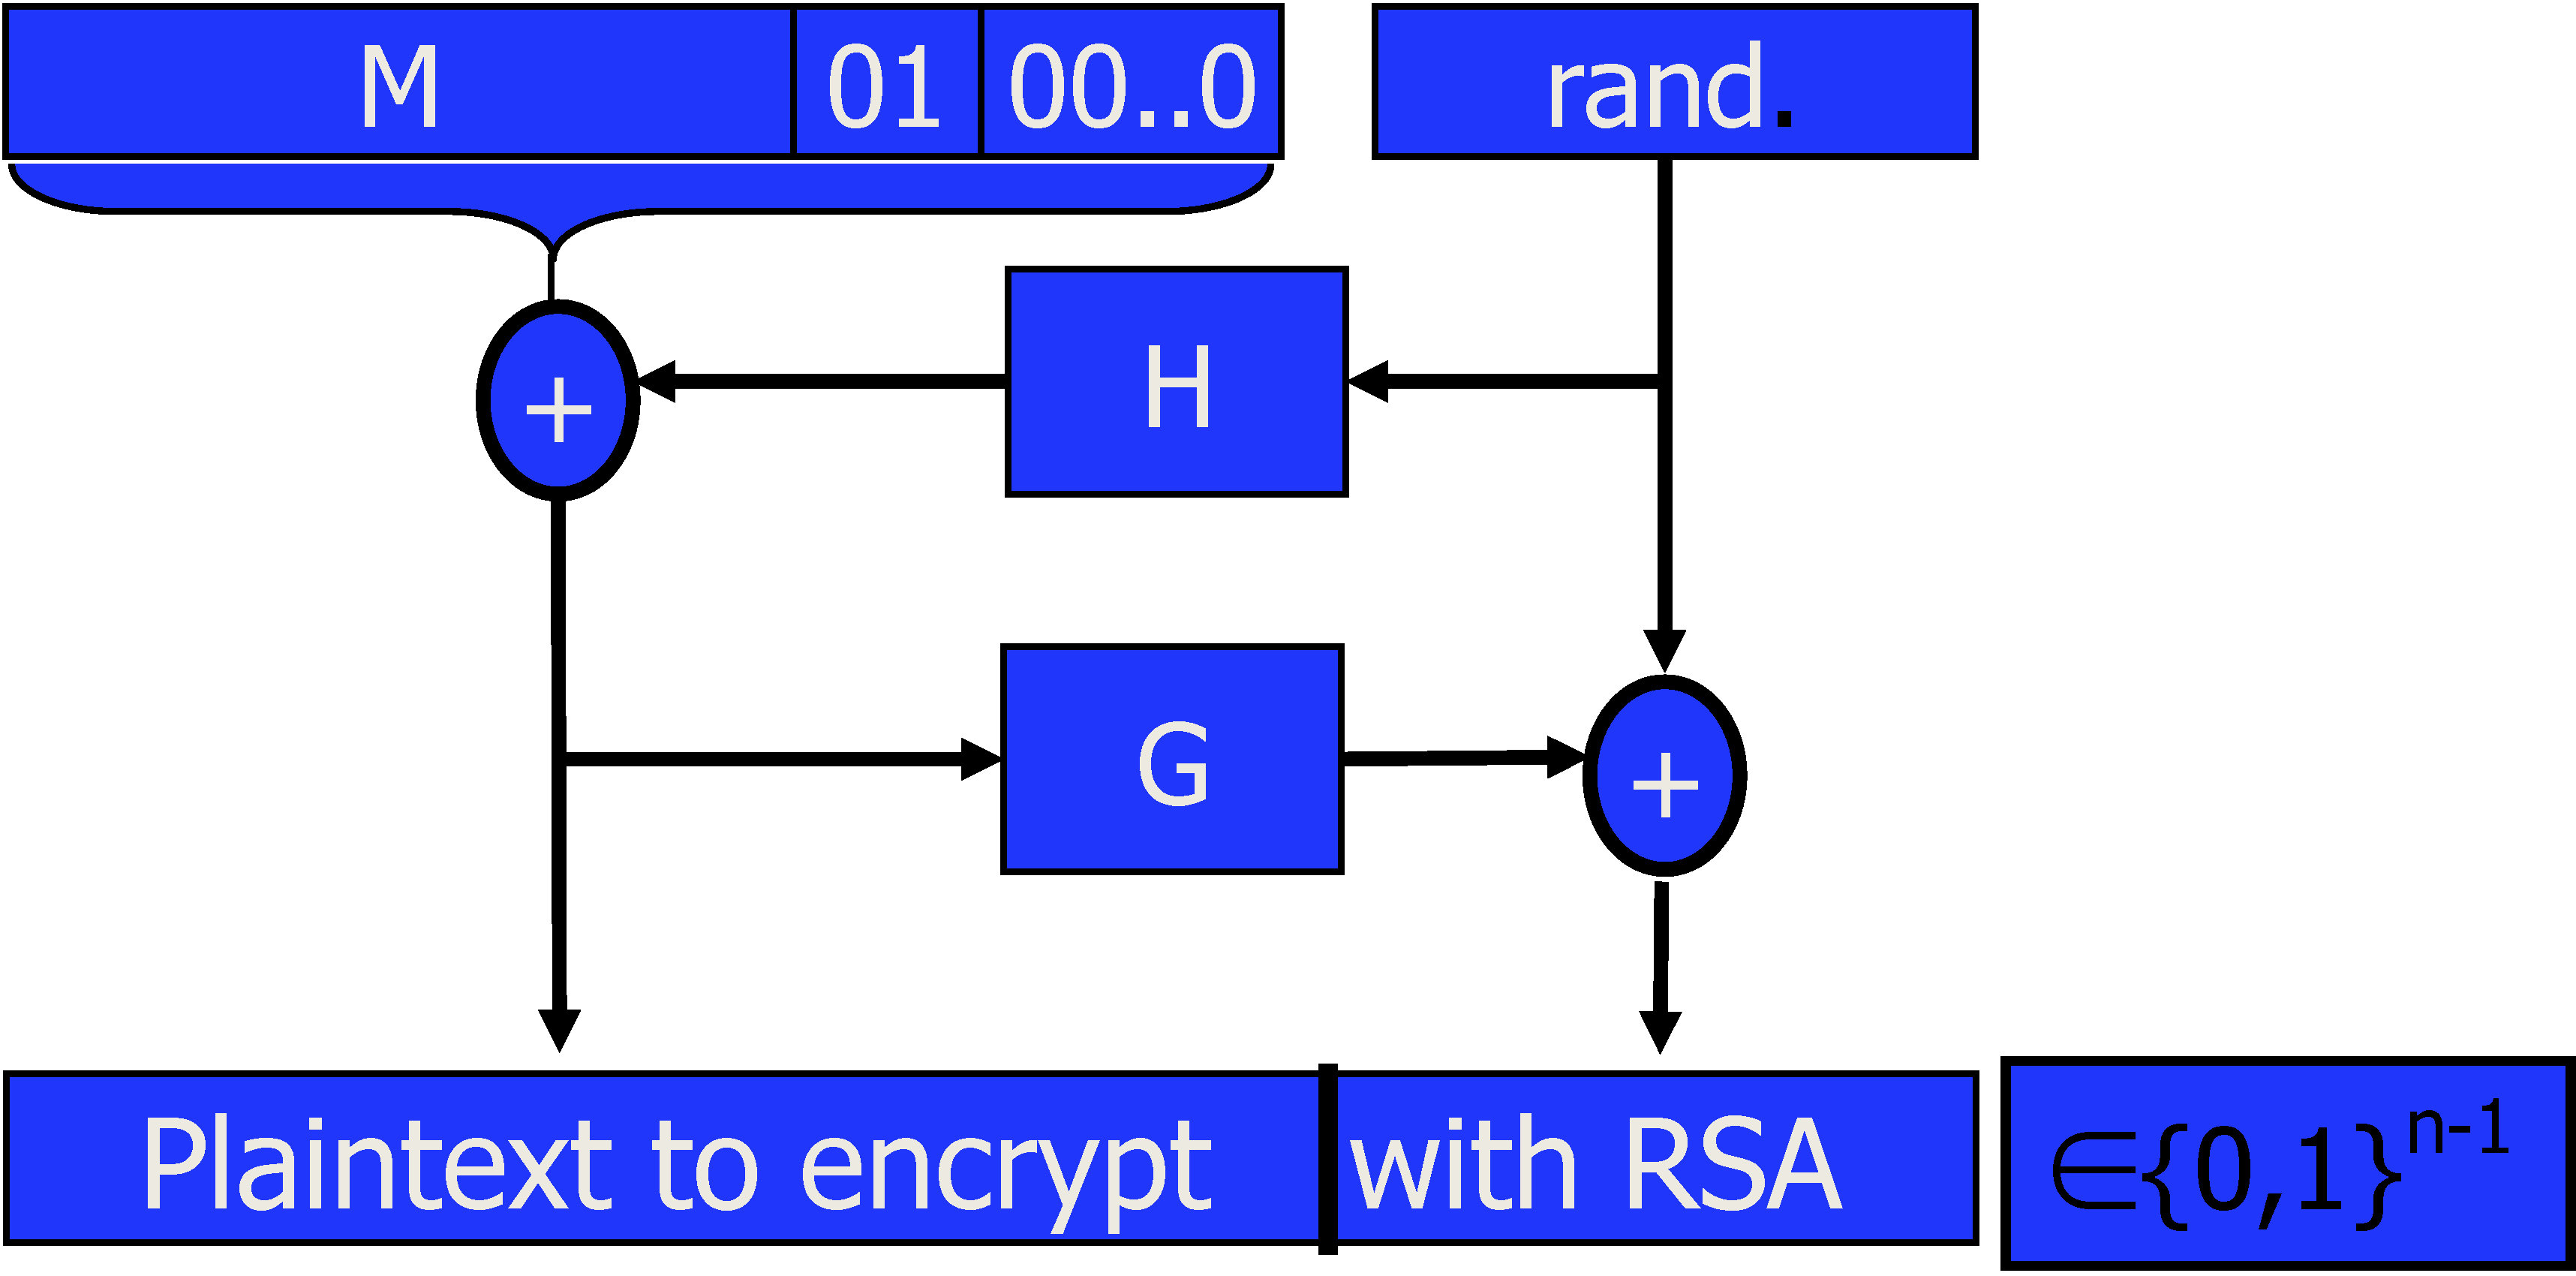
\includegraphics{oaep}
\caption{The OAEP block diagram}
\end{figure}

Theorem: OAEP is \textit{semantically secure} when H, G are \textit{random oracles}. Semantic security means that no partial information (other than the length of the message) is revealed by the ciphertext. The security holds under chosen-plaintext attacks and, when OAEP is used with RSA, under chosen-ciphertext attacks (CCA1) also. 

\section{Random Oracles in Theory and Practice}

Real random oracles don't exist. But the idea is nice: a random oracle $H$ produces outputs $H(x)$ that are truly random but consistent. That is, the oracle always answers any query the same way. We model a random oracle as a function chosen truly randomly from the set of all possible functions [CGH04], where ``possible functions'' are defined as mapping $\{0, 1\}^* \rightarrow \{0,1\}^l,$ where $l$ is the desired output length. 

In practice, random oracles are often implemented using cryptographic hash functions such as SHA1. But systems whose cryptographic security proofs rely on the random oracle model are often not as secure when a hash function is used. Indeed, Canetti, Goldreigh, and Halevi exhibited a crypto-system proven secure under the random oracle model but insecure with any particular implementation of the oracle [CGH04]. 

\section{Implementation Attacks on RSA}
OAEP is important because of vanilla RSA's insecurities. These include both theoretical faults and side-channel attacks on actual software implementations of RSA. 

Several theoretical ways exist to model an adversary. Adversaries may be passive eavesdroppers on the communications channel; they may be able to encrypt messages of their choice (always true in public-key cryptography), in a chosen-plaintext attack; or they may even be able to decrypt ciphertexts of their choice, in a chosen-ciphertext or lunchtime attack. 

In a lunchtime (CCA1) attack, the adversary, Mallory, can request encryptions and decryptions of arbitrary strings (while Alice, the challenger goes to lunch and leaves her computer unattended). Mallory then chooses two messages; Alice selects one at random and encrypts it, and Mallory must say which it is. Because vanilla RSA (without OAEP) is deterministic, Mallory can recognize messages she has already seen, and therefore her task is easy. 

We can formalize the chosen-ciphertext attack as
\begin{align}
  Pr \left[
  \begin{array}{l}
    K \leftarrow \textsf{Gen}(1^n) \\
    (M_0, M_1, \textsf{state}) \leftarrow \mathcal A^{\textsf{Enc}_K(\cdot),\textsf{Dec}_K(\cdot)}(1^n) \\
    B \sim \mathcal U(\{0,1\}) \\
    C^* \leftarrow \textsf{Enc}(K,M_B) \\
    B' \leftarrow \mathcal A^{\textsf{Enc}_K(\cdot)}(1^n,C^*,\textsf{state})
  \end{array}
  : B = B'
  \right]
  < \frac{1}{2} + negl(n).
\end{align}.

A number of attacks on RSA implementations also exist. These include:
\begin{itemize}
	\item Timing attacks, where the number of CPU cycles required to compute $c^d \pmod n$ reveals $d$
	\item Power attacks, where CPU power consumption during computation of $c^d \pmod n$ reveals $d$
	\item Fault attacks, where an error at a critical moment reveals $d$
	\item Cache attacks, where patterns of CPU cache access reveal $d$
\end{itemize}

These are side-channel attacks, where information is revealed by a leaky implementation. Don't roll your own cryto!

\section{Public key cryptography based on squaring}
One other example of a public key cryptosystem, aside from RSA, is based on the squaring function.  More precisely, given a large number $ N $ that is the product of two primes that are each 3 (mod 4), it is hard to find the square root of a given perfect square. (Perfect squares are also called quadratic residues.)  However, it is easier to find such a root given the prime factors $ p $ and $ q $.  This allows us to create the following encryption scheme:
\begin{itemize}
\item Key generation - Generate two large primes $ p $ and $ q $ such that $ p \cong q \cong 3 $ (mod 4).  Keep $ (p,q) $ as the secret key, but announce the public key $ N = pq $.
\item Encryption - $ \mathsf{Enc}(N, m) = c = m^2 $ (mod $ N $)
\item Decryption - $ \mathsf{Dec}(N, c) $ gives the unique square root of $ c $ that is itself a perfect square modulo $ N $.
\end{itemize}
If we know the prime factors $ p $ and $ q $, we can easily find the roots of $ m^2 $ modulo $ N $ by using the Chinese remainder theorem to decompose the problem into finding the roots of $ m^2 $ modulo $ p $ and modulo $ q $.  We know how to find roots modulo primes in polynomial time (see Cipolla's algorithm), and can tell which roots are squares, so we can put this information back together to efficiently find the square root of $ m^2 $ modulo $ N $ that is itself a perfect square.
\\ ~ \\
However, if we don't know $ p $ and $ q $, decrypting is as hard as factorizing $ N $.  In fact, we can find the prime factorization of $ N $ from the roots.  As a result, this encryption scheme is especially vulnerable to lunchtime attacks, which we mentioned earlier.  We will now provide an example of a successful lunchtime attack.
\\ ~ \\
Suppose an attacker had access to the decryption oracle for a short time and found the roots of $ k^2 $ and $ (jk)^2 $ that were quadratic residues, for some $ j $ and $ k $ in $ \mathbb{Z}_N^\ast $.  Suppose $ j $ happened to be a quadratic residue modulo $ p $ but not modulo $ q $.  The roots of $ k^2 $ modulo $ N $ correspond to pairs of roots modulo $ p $ and $ q $, namely $ (k_p, k_q) $, $ (k_p, -k_q) $, $ (-k_p, k_q) $, and $ (-k_p, -k_q) $.  Without loss of generality, say $ k_p $ and $ k_q $ (as opposed to $ -k_p $ and $ -k_q $) are quadratic residues modulo $ p $ and $ q $, respectively.  Then since $ j $ is a quadratic residue modulo $ p $ but not $ q $, $ jk_p $ is a quadratic residue but $ jk_q $ is not; $ -jk_q $ is the quadratic residue instead.
\\ ~ \\
Then the decryption oracle outputs the numbers corresponding to $ (k_p, k_q) $ and $ (jk_p, -jk_q) $.  The Chinese remainder theorem tells us that these numbers are $ pk_q + qk_p $ and $ jqk_p - jpk_q $.  We can divide the second one by $ j $ to get a different root of $ k^2 $, namely $ qk_p - pk_q $.  But now the attacker can add the two roots together to get $ 2qk_p $.  If he takes the greatest common factor of this sum and $ N $, he'll get $ q $, one of the factors, and can find $ p $ from that.  Then, knowing $ p $ and $ q $, the attacker will be able to decrypt messages just as well as the intended recipient.
\\ ~ \\
Since about half the numbers modulo a prime are quadratic residues, and about half aren't, a randomly chosen $ j $ will be a square modulo $ p $ but not $ q $ (or vice versa) about half the time.  This is really bad.  There are, however, ways to protect against such attacks.
\\ ~ \\
This encryption scheme takes $ O(k^2) $ time to encrypt a message and $ O(k^3) $ time to decrypt, where $ k $ is the length of the secret key $ (p, q) $.  This is about the same as RSA.

\section{Single-bit encryption with nondeterministic padding}
In our analyses of cryptosystems thus far, we've assumed that the messages were to be chosen randomly, and proved that our cryptosystem was hard to crack.  But what if the system is easy to crack over the actual message space?
\\ ~ \\
Regardless, we can probably assume that there are approximately the same number of 0's and 1's if we look at our messages bit by bit.  We can randomly pad each bit into a longer string and then encode the string.  The added randomness allows a 0 or 1 to be mapped to one of many strings, so most of the encoded bits look different, even though there are really only two possibilities.
\\ ~ \\
There are two things that we need for this to work: First, we want to be able to undo the random padding to get our original bit back with the aid of a secret key.  Second, we want the bit that we care about (as opposed to all the padding) to be secure against any attacks.
\\ ~ \\
The idea of a string being difficult to decode in general but easy with a secret key suggests that we use a trapdoor function.  In general, we can encrypt a single bit in the manner described with any trapdoor function as follows:
\begin{itemize}
\item Key generation - Pick a trapdoor function $ f $, with secret $ t_f $, and pick a hard-core predicate $ B $ for $ f $.
\item Encryption - To encrypt a bit $ m $, randomly select $ x $ such that $ B(x) = m $, and output $ f(x) =  c $.
\item Decryption - Find $ x = f^{-1}(c) $ with the help of the secret key, and return $ B(x) = m $.
\end{itemize}
This encryption scheme divides the image of $ f $ into strings that correspond to 0 and strings that correspond to 1.  The attacker cannot distinguish which category some $ f(x) $ falls into because $ B $ is a hard-core predicate.

\section{Trapdoor predicates}
These conditions, that $ f $ be a trapdoor function and $ B $ be a hardcore predicate, are a stronger than they need to be.  All that our single-bit encryption scheme really needs to work is that an attacker cannot distinguish between strings that correspond to 0 and those that correspond to 1, but we can.  Also, the scheme would be rather useless if there was no efficient way to encode bits.
\\ ~ \\
This is exactly the definition of a \textit{trapdoor predicate}.  More formally, a trapdoor predicate is a boolean function $ B: \{ 0,1 \}^\ast \Rightarrow \{ 0,1 \} $ that satisfies the following:
\begin{itemize}
\item We need to encrypt efficiently - There is a probabilistic polynomial-time algorithm $ \mathcal{A} $ that outputs random $ x $ such that $ B(x) = m $, the bit we are trying to encode.
\item We need our bit to be secure - For any probabilistic polynomial-time algorithm $ \mathcal{B} $, we want $ \text{Pr}[\mathcal{B}(x) = B(x)] < \frac{1}{2} + p(k) $ for any non-negligible function $ p $.
\item We need to be able to decode - Given some secret key $ s $, we need to be able to compute $ B(x) $ in probabilistic polynomial-time.
\end{itemize}
~ \\
Now let's look at an example of a trapdoor predicate.  We'll use a scheme similar to the squaring scheme given above, based on a similar problem of trying to distinguish quadratic residues from nonresidues.
\begin{itemize}
\item Key generation - Generate two large primes $ p $ and $ q $ such that $ p \cong q \cong 3 $ (mod 4).  Keep $ (p,q) $ as the secret key, but announce the public key $ N = pq $.  (Just like before.)
\item Encryption - For our message bit $ m $, randomly generate $ x \in \mathbb{Z}_N^\ast $ and output $ \mathsf{Enc}(N, m) = (-1)^mx^2 = c $.  Now since -1 is a nonresidue, $ c $ is a quadratic residue if and only if $ m = 0 $.
\item Decryption - Decide whether $ c $ is a quadratic residue, and return 0 if it is and 1 if it's not.
\end{itemize}
We can use the same algorithm as before to determine whether $ c $ is a quadratic residue or not, if we know $ p $ and $ q $: just try to take the square root and if there aren't any, it's not a perfect square.  But if we don't know $ p $ and $ q $, figuring out whether $ c $ is a quadratic residue or not is just as hard as actually finding the roots.  And earlier we realized that this is as hard as factoring $ N $, which is a very hard problem!

\section{Using single-bit encryption for arbitrary length encryption}

Now that we can encrypt single bits, can we encrypt a multibit message bit-by-bit and expect security? The answer is yes!

Let $\Pi = (\textsf{Gen, Enc, Dec})$ be a semantically secure probabilistic encryption scheme for single bits. Then define \textit{probabilistic encryption} $PE_\Pi = (\textsf{G, E, D})$ as follows:

\begin{itemize}
  \item $G(1^k) = Gen(1^k)$
  \item $E(pk, m = m_1 \cdots m_l) = Enc(pk, m_1) \cdots Enc(pk, m_l)$: bit-by-bit encryption
  \item $D(sk, c = c_1 \cdots c_l) = Dec(sk, c_1) \cdots Dec(sk, c_l)$: bit-by-bit decryption
\end{itemize}

\begin{theorem}
  If $\Pi = (\textsf{Gen, Enc, Dec})$ is semantically secure for single bits, then $PE_\Pi$ is semantically secure for messages of any length.
\end{theorem}

Proof: The proof is by hybridization. Suppose there existed a probabilistic polynomial time adversary algorithm $\mathcal A$ and a message space $\mathcal M$ with $l$ bit messages, such that over a random choice of two messages $m_0$ and $m_1$ from $\mathcal M$ and a random encryption of one of those messages $c$,
\begin{align}
  P[\mathcal A(e, m_0, m_1, c) = m] > \frac{1}{2} + \frac{1}{P(k)}
\end{align}
for infinitely many $k$ and some polynomial $P.$ (That is, the adversary can frequently guess with nonnegligible probability which of two messages has been encrypted.)

Then we can use this adversary to decrypt, with non-negligible probability, single encrypted bits as follows. 

The existence of $\mathcal A$ implies that for infinitely many message lengths $k$, $\mathcal A$ can distinguish between encrypted random $m_0^k, m_1^k \in \mathcal M$ with better than negligible probability over (a) choice of encryption keys and (b) the probabilistic ciphertexts $c_1 = E(e, m_1^k), c_2 = E(e, m_2^k)$.

Now pick a $k$ such that $\mathcal A$ can distinguish messages generated from the space $\mathcal M(1^k)$ well:
\begin{align}
  P[A(e, c_0) = 1] - P[A(e, c_1) = 1] > \alpha \text{ over} \\
  (e,d) \in G(1^k), \\
  c_0 \in E(e, m_0^k), \\
  c_1 \in E(e, m_1^k).
\end{align}

We are now ready to receive our encrypted bit $c,$ encrypted with public key $e$.
\begin{enumerate}
  \item Choose two messages, $m_0^k, m_1^k,$ of length $l,$ whose ciphertexts $\mathcal A$ can distinguish. Without loss of generality, assume that $A$ outputs $1$ more often on message $m_1^k$ than on $m_0^k.$
  \item Construct a series of hybrid messages $s_i$, where $s_i$ consists of the first $i$ bits of $m_0^k$ and the last $l - i$ bits of $m_1^k.$ We know that
  \begin{align}
    \sum_{i = 1}^l (P[A(e, Enc(e, s_{i+1}) = 1] - P[A(e, Enc(e, s_i)) = 1]) > \alpha
  \end{align}
  
  Therefore, there must be some particular $i$ such that
  \begin{align}
    P[A(e, Enc(e, s_{i+1})) = 1] - P[A(e, Enc(e, s_i)) = 1] > \frac{\alpha}{l}
  \end{align}
  
  Generate a ciphertext $(c_1, \cdots, c_l) = Enc(e, s_i)$ and stick our mystery encrypted bit $c$ in position $i$. Then compute $b = A(c_1, \cdots, c, \cdots, c_l)$ and output the $i$th bit of $m_1^k$ if $b = 1$ or the $i$th bit of $m_0^k$ if $b = 0.$
\end{enumerate}

If $\mathcal A$ exists, then the above algorithm decrypts single bits with nonnegligible probability, which contradicts our assumption that our single-bit probabilistic scheme achieved semantic security. Therefore, the multi-bit scheme is semantically secure also. 

\section{Homomorphic encryption}

\begin{definition}An encryption scheme is \textbf{homomorphic} if computations on the ciphertexts are reflected as computations on the messages when decrypted.\end{definition}

Symbollically, given an encryption function $E$ and messages $m_1$ and $m_2$, this means
\begin{align*}
E(m_1) \circ E(m_2) &= E(m_1 \diamond m_2).
\end{align*}
Note that the operation on the cyphertexts and the messages can be different operations. Example applications of homomorphic encryption schemes:
\begin{itemize}
	\item E-voting: all votes could be encrypted and include a 0 or 1 indicating the vote. The ciphertexts of the votes could be added and then decrypted, yielding the vote count without revealing individual votes.
	\item Secure cloud computing: data could be encrypted and have ciphertexts operated on (both $+$ and $\times$) without revealing the data itself. The result would then be decrypted and used.
\end{itemize}
Specifically with the quadratic residuosity encryption scheme, we have the following homomorphic properties:
\begin{itemize}
	\item $E(m_1 \oplus m_2) = E(m_1) \cdot E(m_2)$ (can be checked with truth table)
	\item $E(1 \oplus m) = E(1) - E(m)$
	\item $E(m) = E(0) \cdot E(b)$ (effectively re-randomizing)
\end{itemize}





\section{Probabilistic encryption scheme and examples}

\subsection{Main Idea}

Given a trapdoor permutation collection $F$, we define an encryption scheme as follows:
\begin{itemize}
	\item The key generation function $\gen(1^k)$ simply chooses a $f\in F$ and its corresponding trapdoor $t$, and outputs $(f, t)$.
	\item The encryption function $\enc(f, m)$ chooses a seed $r$ in the domain of $f$ and a PSRG $g$ based on $f$. It returns $c = (c_1, c_2) = (g(r)\oplus m, f^{|m|+1}(r))$.
	\item The decryption function $\dec(t, (c_1, c_2))$ has access to the trapdoor. It first finds $r = f^{-(|m|+1)}(c_2)$ (by inverting over and over) then returns $m=c_1 \oplus g(r)$.
\end{itemize}
The security of this scheme follows from the assumption of a PSRG.

\subsection{Example: RSA}

The probabilistic approach can be applied to RSA as follows:
\begin{itemize}
	\item $\gen(1^k)$ is defined as choosing $(n,e)$ just as in RSA.
	\item $\enc(n,m)$ is defined by choosing $r \in Z_n^{*}$ and concatenating $|m|$ bits computed by
	\begin{align*}
	\text{pad} &= \text{lsb}(r \text{ mod } n) \quad \text{lsb}(r^e \text{ mod } n) \quad  \text{lsb}(r^{e^2} \text{ mod } n) \quad  \cdots \quad  \text{lsb}(r^{e^{|m|-1}} \text{ mod } n).
	\end{align*}
	We then set $c=( \text{pad} \oplus m, r^{|m|})$.
	\item $\dec((p,q),(c_1, c_2))$ decrypts by finding $r$ as the $|c_1|$th root of $c_2$ modulo $n$ (using the factorization $n=pq$). Then, it can recompute $\text{pad}$ as above and find $m = c_1 \oplus \text{pad}$.
\end{itemize}

\subsection{Example: El Gamal}

The El Gamal Cryptosystem is based on the discrete log problem and takes advantage of probabilistic encryption, defined as follows:
\begin{itemize}
	\item $\gen(1^k)$ chooses a random $k$-bit prime $p$ such that $p=2q+1$, where $q$ is also prime. Let $g$ be a generator of $QR_p$, $x$ be a number with $1 < x < q$, and $y = g^x \mod p$. Publish $(p,g,y)$ as the public key and keep the $x$ that was used secret.
	\item $\enc((p,g,y),m)$ (where $m \in QR_p$) is defined by choosing randomly $1 \le r \le q$, computing $\text{pad} = y^r = g^{xr} \mod p$, and yielding $c = (\text{pad} \cdot m \mod p, g^{r})$.
	\item $\dec(x,(c_1, c_2))$ is able to decrypt the cipher by recomputing the pad as $\text{pad} = c_2^x = g^{rx} \mod p$ and finding $m = c_1 \cdot \text{pad}^{-1} \mod P$. by finding $r$ as the $|c_1|$th root of $c_2$ modulo $n$ (using the factorization $n=pq$). Then, it can recompute $\text{pad}$ as above and find $m = c_1 \oplus \text{pad}$.
\end{itemize}
Note that $g$ and $p$ can be shared across all the users as long as $x$ and therefore $y$ are chosen differently for each key generation. 

This scheme has, for message size $|m| = k$, public key of size $O(k)$, bandwidth of $O(k)$, and both encryption and decryption running time of $O(k^3)$. We also have security:
\begin{theorem}
Under DDH, El Gamal is computationally indistinguishable.
\end{theorem}

El Gamal also has multiplicative homomorphism. That is, if $\enc(m) = (c_1, c_2)$ and $\enc(m') = (c_1', c_2')$, we have $\enc(m \cdot m') = (c_1c_1' \mod p, c_2c_2' \mod p)$. 

Furthermore, we can modify the scheme to also have additive homomorphism as follows. In encrypting, instead of returning $c_1 = \text{pad} \cdot m \mod p$, we set $c_1 = \text{pad} \cdot g^m \mod p$. With this modification, multiplying $g^m \cdot g^{m'} = g^{m+m'}$ effectively adds $m+m'$. To decrypt, as long as $m$ is a member of a polynomial size known set, can try all possibilities for $g^m$ and choose the one that matches.

\subsection{Example: Paillier}

Another example of an encryption scheme that uses randomness is as follows:

\begin{itemize}
	\item $\gen(1^k)$ chooses a $n=pq$, where $p$ and $q$ are primes. It publishes $n$ and keeps $\phi(n)$ secret.
	\item $\enc(n,m)$ (assuimg $m \in Z_n^*$) chooses a random $r \in Z_n^*$ and computes
	\begin{align*}
	c &= (1+n)^mr^n \mod n^2.
	\end{align*}
	\item $\dec((p,q),c)$ first computes
	\begin{align*}
	c' &= c^{\phi(n)} \mod n^2 \\
	&= (1+n)^{m \phi(n)} r^{n \phi(n)} \mod n^2 \\
	&= (1+n)^{m \phi(n)} \mod n^2 \\
	&= 1+nm \phi(n) \mod n^2,
	\end{align*}
	from which we can find $m = \frac{c'-1}{n \phi n}$.
\end{itemize}
Note that the last step of decryption follows from the fact $(1+n)^t = 1 + tn + n^2 ( \cdots ) = 1+tn \mod n^2$ for any $t$.

The Paillier encryption scheme is used in applications such as auctions and voting due to its homomorphic properties: if $\enc(n, m) = c$ and $\enc(n, m') = c'$, then $\enc(n, m+m' \mod n) = c \cdot c'$ and $\enc(n, m-m' \mod n) = c / c'$.

The security of the scheme is guaranteed under the Decisional Composite Residuosity (DCR) assumption. 
\begin{definition}
	The Decisional Composite Residuosity (DCR) assumption states that it is hard to distinguish between $(n, R^n)$ and $(n, S)$ for random $R \in Z_n$ and $S \in Z_{n^2}$.
\end{definition}
\noindent With DCR, Paillier is computationally indistinguishable against a passive adversary.

% % % You should probably leave the below alone % % %
\nocite{*}
\bibliographystyle{alpha}
\bibliography{scribe-bib}
\end{document}
